\subsection{Hệ tọa độ và các hệ tọa độ phổ biến}

\begin{frame}{Ý nghĩa của hệ tọa độ}
    \begin{columns}
        \column{0.32\textwidth}
        \begin{itemize}
            \item Xác định vị trí các vật trong không gian.
            \item Các trục, biến tọa độ được tùy chọn phù hợp với từng ví dụ.
            \item Các hệ tọa độ trực giao thường được ưu tiên sử dụng với các hệ phức tạp.
        \end{itemize}
        \column{0.68\textwidth}
        \vspace{-4mm}
        \begin{figure}
            \centering
            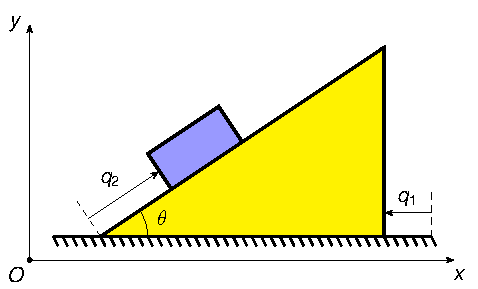
\includegraphics[width=0.9\linewidth]{Figures/Sliding_wedge.pdf}
            \caption{Nhiều hệ tọa độ khác nhau cho bài toán nêm trượt trên nêm}
            \label{fig:Sliding_wedge}
        \end{figure}
    \end{columns}
\end{frame}

\begin{frame}{Các hệ tọa độ 3 chiều phổ biến}
    \vspace{-4mm}
    \begin{columns}
        \column{0.33\textwidth}
        \begin{itemize}
            \item Hệ tọa độ Dercates
        \end{itemize}
        \begin{figure}
            \centering
            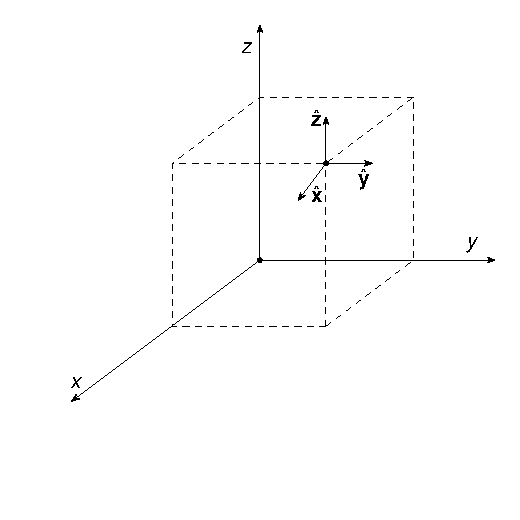
\includegraphics[width=\linewidth]{Figures/Decartes_coordinate.pdf}
            \caption{Hệ tọa độ Decartes.}
            \label{fig:Decartes_coordinate}
        \end{figure}

        \column{0.33\textwidth}
        \begin{itemize}
            \item Hệ tọa độ trụ
        \end{itemize}
        \begin{figure}
            \centering
            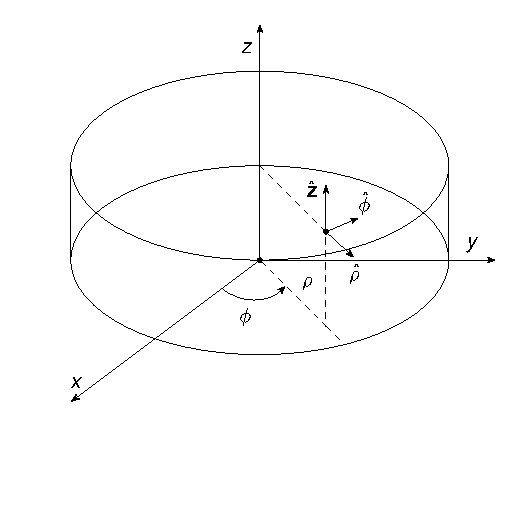
\includegraphics[width=\linewidth]{Figures/Cylindrical_coordinates.pdf}
            \caption{Hệ tọa độ trụ.}
            \label{fig:Cylindrical_coordinates}
        \end{figure}

        \column{0.33\textwidth}
        \begin{itemize}
            \item Hệ tọa độ cầu
        \end{itemize}
        \begin{figure}
            \centering
            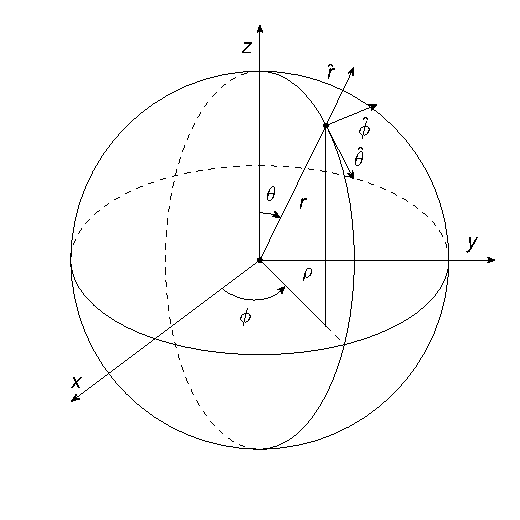
\includegraphics[width=\linewidth]{Figures/Spherical_coordinate.pdf}
            \caption{Hệ tọa độ cầu.}
            \label{fig:Spherical_coordinate}
        \end{figure}

    \end{columns}

\end{frame}

\begin{frame}{Tọa độ Frenet - Serret}
    \begin{columns}
        \column{0.33\textwidth}
            Tên gọi
            \begin{itemize}
                \item Vector đơn vị tiếp tuyến \(\mathbf{T}\).
                \item Vector đơn vị pháp tuyến \(\mathbf{N}\).
                \item Vector đơn vị trực chuẩn \(\mathbf{B}\).
            \end{itemize}
        \column{0.33\textwidth}
            Định nghĩa:
            \begin{align}
                \mathbf{T} & := \frac{\mathrm{d} \mathbf{r}}{\mathrm{d} s}, \\
                \mathbf{N} & := \frac{\mathrm{d} \mathbf{T} / \mathrm{d} s}{\left\| \mathrm{d} \mathbf{T} / \mathrm{d} s \right\|}, \\
                \mathbf{B} & := \mathbf{T} \times \mathbf{N}.
            \end{align}
        \column{0.33\textwidth}
            Công thức Frenet Serret
            \begin{align}
                \frac{\mathrm{d} \mathbf{T}}{\mathrm{d} s} &= \kappa \mathbf{N}, \\
                \frac{\mathrm{d} \mathbf{N}}{\mathrm{d} s} &= - \kappa \mathbf{T} + \tau \mathbf{B}, \\
                \frac{\mathrm{d} \mathbf{B}}{\mathrm{d} s} &= - \tau \mathbf{N}.
            \end{align}
    \end{columns}
    \begin{columns}
        \column{0.33\textwidth}
        \begin{itemize}
            \item Độ cong \(\kappa\).
            \item Bán kính cong \(R_c = 1/\kappa\).
            \item Độ xoắn đường cong không gian \(\tau\).
        \end{itemize}
        \column{0.67\textwidth}
        \vspace{-2mm}
        \begin{figure}
            \centering
            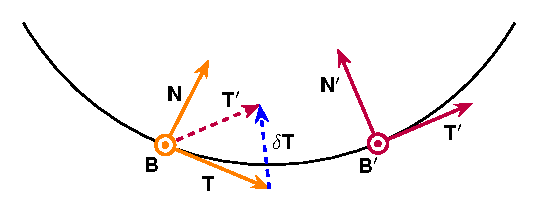
\includegraphics[width=0.7\linewidth]{Figures/Frenet_Serret.pdf}
            \vspace{-2mm}
            \caption{Các vector đơn vị trên hệ tọa độ cong.}
            \label{fig:Frenet_Serret}
        \end{figure}
    \end{columns}
\end{frame}

\subsection{Độ cong và bán kính cong}

\begin{frame}{Tính toán bán kính cong trong không gian 2 chiều - đường cycloid}
    \begin{columns}
        \column{0.6\textwidth}
            Độ cong:
            \begin{equation}
                \kappa = \dfrac{\mathrm{d} \phi}{\mathrm{d} s} = \frac{x' y" - y' x"}{\left( x'^2 + y'^2 \right)^{3/2}}
            \end{equation}
            Bán kính cong \(R_c = 1/\kappa\), tính toán với đường cycloid
            \begin{equation}
                R_c = 4 R \cos \left( \dfrac{\theta}{2} \right).
            \end{equation}
            Tại điểm cao nhất, \(\theta=0\), \(R_c=4R\).
            \begin{itemize}
                \item Bán kính cong là bán kính của đường tròn khớp nhất so với quỹ đạo tại điểm được khảo sát. \cite{BoiDuoongHSGTHPT_Phantich}
            \end{itemize}
        \column{0.4\textwidth}
        \vspace{-7mm}
        \begin{figure}
            \centering
            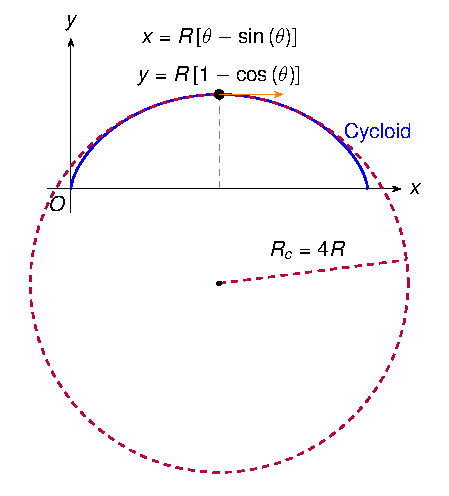
\includegraphics[width=0.9\linewidth]{Figures/Cycloid.pdf}
            \caption{Quỹ đạo Cycloid và bán kính cong tại điểm cao nhất trên quỹ đạo.}
            \label{fig:Cycloid}
        \end{figure}
    \end{columns}
\end{frame}

\subsection{Chuyển động ném xiên}

\begin{frame}{Chuyển động ném xiên}
    \begin{columns}
        \column{0.5\textwidth}
        \vspace{-3mm}
            \begin{itemize}
                \item Điều kiện đầu: \\
                \(x(0)=0\), \(y(0)=0\), \(\dot{x}(0)= v_0 \cos \alpha\), \(\dot{y}(0)= v_0 \sin \alpha\).
                \item Phương trình vi phân chuyển động: \(\ddot{x} = 0\), \(\ddot{y} = -g\).
                \item Nghiệm:
                \begin{align}
                    x(t) &= v_0 \cos \left( \alpha \right) t, \\
                    y(t) &= v_0 \sin \left( \alpha \right) t - \frac{1}{2} g t^2 \\
                    y(x) &= x \tan \left( \alpha \right) - \frac{v_0^2}{2g \cos^2 \left( \alpha \right)}x^2. 
                \end{align}
            \end{itemize}            
        \column{0.5\textwidth}
            \vspace{-2mm}
            \begin{figure}
                \centering
                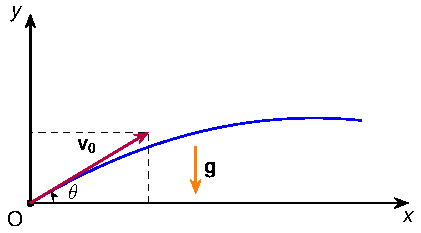
\includegraphics[width=0.9\linewidth]{Figures/Projectile_motion.pdf}
                \caption{Bài toán chuyển động ném xiên, các điều kiện đầu và quỹ đạo của vật.}
                \label{fig:Projectile_motion}
            \end{figure}
            \vspace{-5mm}
            \begin{itemize}
                \item Bài tập: Xác định độ cong và bán kính cong của quỹ đạo tại thời điểm \(t\).
            \end{itemize}
    \end{columns}
\end{frame}

\subsection{Bài toán đuổi bắt}

\begin{frame}{Bài toán đuổi bắt - 1: Rùa đuổi nhau}
    \begin{columns}
        \column{0.3\textwidth}
            Giải
            \begin{align*}
                r \frac{\mathrm{d} \theta}{\mathrm{d} r} &= -1 \\
                \int_{a/\sqrt{2}}^r \frac{\mathrm{d} r}{r} &= - \int_{\pi/4}^\theta \mathrm{d} \theta  \\
                \Rightarrow r &= \frac{a}{\sqrt{2}} \exp \left( \frac{\pi}{4} -\theta \right).
            \end{align*}

            \begin{itemize}
                \item Tỷ lệ vàng!!!
            \end{itemize}
        \column{0.7\textwidth}
        \begin{figure}
            \centering
            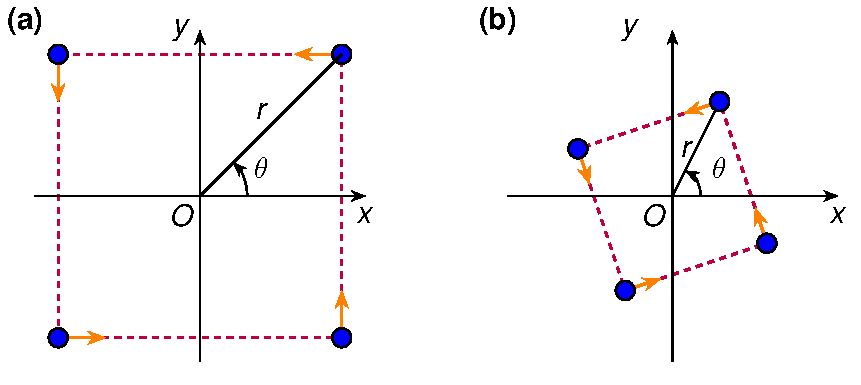
\includegraphics[width=0.9\linewidth]{Figures/Turtles_ninja.pdf}
            \caption{4 con rùa đuổi bắt: \textbf{(a)} Thời điểm ban đầu, \textbf{(b)} Tại một thời điểm bất kỳ}
            \label{fig:Turtles_ninja}
        \end{figure}
    \end{columns}
\end{frame}

\begin{frame}{Bài toán đuổi bắt - 2: Chó đuổi thỏ}
    \begin{columns}
        \column{0.3\textwidth}
            Viết phương trình vi phân đối với hai hệ tọa độ khác nhau:
            \begin{itemize}
                \item Tọa độ Decartes \( \left( x, y \right) \).
                \item Toạ độ cực \( \left( r, \theta \right) \). \cite{brebec2005cohoc1}
            \end{itemize}
        \vspace{5mm}
        \textit{Giải phương trình vi phân của bài toán này sẽ là một câu chuyện khác...}
        \column{0.7\textwidth}
        \vspace{-5mm}
        \begin{figure}
            \centering
            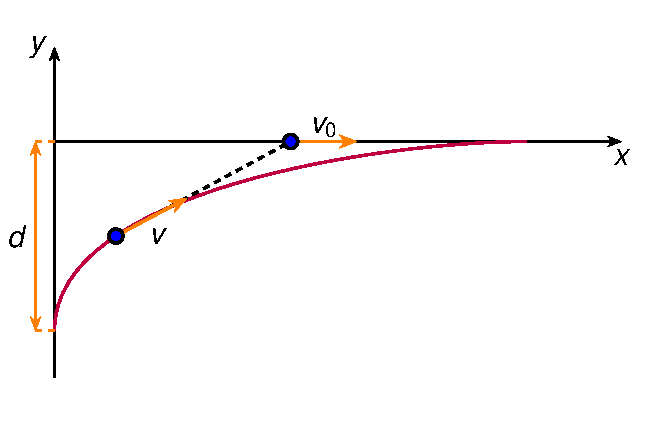
\includegraphics[width=0.9\linewidth]{Figures/Pursuit.pdf}
            \vspace{-2mm}
            \caption{Chó vận tốc \(v\) đuổi theo thỏ chuyển động thẳng vận tốc \(v_0\).}
            \label{fig:Pursuit}
        \end{figure}
    \end{columns}
\end{frame}

